\documentclass[preprint, floatfix, pra, showpacs, showkeys]{revtex4}
\usepackage{graphicx}
\usepackage{dcolumn}

\newcommand{\threej}[6]{\ensuremath{\left({#1\atop #4}{#2\atop #5}
{#3\atop #6}\right)}}
\newcommand{\sixj}[6]{\ensuremath{\left\{{#1\atop #4}{#2\atop #5}
{#3\atop #6}\right\}}}

\begin{document}

\title{The Flexible Atomic Code: II. Electron Impact Excitation} 
\author{Ming Feng Gu}
\affiliation{Center for Space Research, Massachusetts Institute of Technology,
Cambridge, MA 02139} 
\email[Email: ]{mfgu@space.mit.edu}

\begin{abstract}
An efficient implementation of the relativistic distorted wave approximation
for the calculation of direct excitation by electron impact is
described. Using the factorization-interpolation method, the calculation of
the collision strengths
for a given array of transitions is very rapid. We pay special attention to
the long range contributions to the continuum-continuum radial
integral by using the phase-amplitude method for the continuum
wavefunctions. The contributions from large angular momentum partial waves
for the allowed transitions are taken into account by the Coulomb-Beth
approximation. The results for some $2\to 3$ transitions of Ne-like iron and
$2\to 2$ transitions of Be-like iron are presented and compared with previous
works.
\end{abstract}

\pacs{34.80.Kw}
\keywords{Distorted-wave; Collision strength}
\maketitle

\section{Introduction}
This is the second of a sequence of papers describing a complete software
package for calculating various atomic processes, the Flexible Atomic Code
(FAC). The present paper deals with the calculation of electron impact
excitation (EIE) in the distorted-wave (DW) approximation. EIE is an important
line formation process in hot plasmas frequently encountered in laboratory
experiments and astrophysics. Accurate cross sections are needed for the
calculation of level populations and line emissivities. 

Two classes of methods are commonly used in the calculation of EIE cross
sections. The first is based on a set of close-coupling (CC) equations, which
takes into account the coupling of various excitation channels
\cite{seaton75}. In these methods, resonances can be included in a
natural way by including the coupling to closed channels. Several
implementations of this method exist. The most widely used is the R-matrix
code developed by a group at the Queens University of Belfast
\cite{berrington95}. The second class of methods is based on the first order
Born approximation, which assumes independent excitation channels. The
coupling to closed channels, which results in resonances, may be included in a
perturbative fashion \cite{eissner72}. Different variants exist according to
the different treatments of the continuum wavefunctions. The plane-wave (PW)
Born approximation uses an unperturbed plane wave for the free orbital. The
Coulomb-wave (CW) Born approximation takes into account the distortion of the
continuum due to a pure Coulomb potential. The most accurate of this class is
the DW Born approximation, in which the free orbitals are
calculated in a more realistic potential taking into account the electronic
structure of the target ion.
The majority of the computer programs in this class implement the DW
approximation, since it yields significantly better results than the PW and CW
methods with minimal increase in the complexity. Many DW codes are in use
today. For example, the non-relativistic DW code from University College
London \cite{eissner98}, the relativistic code of \textcite{hagelstein87}, the
HULLAC package \cite{barshalom88}, the code by \textcite{zhang89}, and that of
\textcite{chen96}, just to name some. The present DW implementation in FAC is
in principle similar to any of the relativistic codes listed above.

In the present implementation, the factorized formula of the collision
strength is used, which separates the angular integration from the radial
integrals, and permits efficient interpolation of the radial integrals. To
avoid the difficulties in the radial integration arising from the oscillatory
behavior of the continuum wavefunctions, we use a different technique from
that for bound orbitals to solve the Dirac equation for free electrons. In the
inner region where the wavefunction is not oscillatory or when one oscillation
period contains 
a sufficient number of radial grid points to ensure the accuracy of numerical
integration, we use the standard Numerov method to integrate the equation 
outward. In the outer region, a phase-amplitude method is used. The position
where the outer solution is matched to the inner solution depends on the
energy and angular momentum of the continuum orbital. This method allows us to
evaluate the radial integrals involving the continuum orbitals to sufficiently
large radial distance without using a prohibitively dense grid. The collision
strength is calculated using the standard partial wave summation. A
quasi-logarithmic grid is constructed for the orbital angular momenta of the
free electrons. Detailed calculations are only carried out on this
grid. Partial collision strengths for all other orbital angular momenta are
obtained by interpolation. Very large
angular momentum contributions to the allowed transitions
are taken into account by the rapid Coulomb-Bethe approximation
\cite{burgess74}. 

In Section \ref{sec_theory} we outline the theoretical background, present the
factorized formula of collision strengths, and discuss the numerical
techniques used to solve the continuum Dirac equation and perform the partial
wave summation. Section \ref{sec_results} illustrates the correctness of the
program by calculating collision strengths of some $2\rightarrow 3$
transitions in Ne-like iron and $2\to 2$ transitions in Be-like iron. The
results are found to agree with existing publications. Section
\ref{sec_conclusions} gives a brief summary.

\section{Theory and Numerical Techniques}
\label{sec_theory}
\subsection{Factorized Collision Strength}
The EIE cross section $\sigma_{01}$ from the inital state $\psi_0$ to the final
state $\psi_1$ can be expressed in terms of the collision strength
$\Omega_{01}$ as (in atomic units, which we shall use throughout the
paper) 
\begin{equation}
\sigma_{01} = \frac{\pi}{k_0^2g_0}\Omega_{01},
\end{equation}
where $g_0$ is the statistical weight of the initial state, and $k_0$ is the
kinetic momentum of the incident electron, which is related to the energy
$\varepsilon_0$ by
\begin{equation}
k_0^2 = 2\varepsilon_0\left(1+\frac{\alpha^2}{2}\varepsilon_0\right),
\end{equation}
where $\alpha$ is the fine structure constant. The continuum wavefunction
is normalized so that the large component has an asymptotic amplitude of
$\sqrt{k/\varepsilon}$, which reduces to $\sqrt{2/k}$ in the non-relativistic
limit, or equivalently,
\begin{equation}
\int_0^\infty \left[P_{\varepsilon(r)}P_{\varepsilon^\prime}(r)
+Q_{\varepsilon(r)}Q_{\varepsilon^\prime}(r)\right]d r = 
\pi\delta(\varepsilon - \varepsilon^\prime),
\end{equation}
where $\varepsilon$ and $k$ are the energy and kinetic momentum of the
orbital, $P_\varepsilon$ and $Q_\varepsilon$ are the large and small
components of the continuum wavefunction. The collision strength can be
written as
\begin{equation}
\Omega_{01} = 2\sum_{\kappa_0\kappa_1}\sum_{J_T}[J_T]
|<\psi_0\kappa_0,J_TM_T|\sum_{i<j}\frac{1}{r_{ij}}|\psi_1\kappa_1,J_TM_T>|^2,
\end{equation}
where $\kappa_0$ and $\kappa_1$ are the relativistic angular quantum numbers of
the incident and scattered electrons, $J_T$ is the total angular momentum
when the target state is coupled to the continuum orbital, $M_T$ is the
projection of the total angular momentum, and  $[J] = 2J+1$. 
Following \textcite{barshalom88}, this expression can be simplified to give
\begin{equation}
\label{eq_cs}
\Omega_{01} = 2\sum_{k}\sum_{\alpha_0\alpha_1\atop\beta_0\beta_1}
Q^k(\alpha_0\alpha_1;\beta_0\beta_1)
<\psi_0||Z^k(\alpha_0,\alpha_1)||\psi_1>
<\psi_0||Z^k(\beta_0,\beta_1)||\psi_1>,
\end{equation}
where 
\begin{equation}
\label{eq_Qk}
Q^k(\alpha_0\alpha_1;\beta_0\beta_1) = \sum_{\kappa_0\kappa_1}[k]^{-1}
P^k(\kappa_0\kappa_1;\alpha_0\alpha_1)P^k(\kappa_0\kappa_1;\beta_0\beta_1),
\end{equation}
and 
\begin{equation}
\label{eq_Pk}
P^k(\kappa_0\kappa_1;\alpha_0\alpha_1)=
X^k(\alpha_0\kappa_0;\alpha_1\kappa_1)+\sum_{t}
(-1)^{k+t}[k]\sixj{j_{\alpha_0}}{j_1}{t}{j_0}{j_{\alpha_1}}{k}
X^t(\alpha_0\kappa_0;\kappa_1\alpha_1),
\end{equation}
where $X^k$ and the operator $Z^k(\alpha,\beta)$ are defined in
Ref.~\cite{gu02a}. 
 
The importance of Eq.~(\ref{eq_cs}) is that the angular and radial integrals
are completely factorized. The radial integrals
$Q^k(\alpha_0\alpha_1;\beta_0\beta_1)$ with the same set of bound orbitals
$\alpha_0$, $\alpha_1$, $\beta_0$, and $\beta_1$ may appear in many
transitions. These integrals also depend on the energy of incident
and scattered electrons, or for a fixed scattered electron energy, they depend
on the excitation energy of the transition $\Delta E$. However, as noted by
\textcite{barshalom88}, the dependence on $\Delta E$  is rather weak. For
dipole forbidden radial integrals, $Q^k \propto \Delta E$, and for dipole
allowed integrals, $Q^k \propto \ln\Delta E$ approximately holds over a wide
range of transition energes. Therefore, for a given scattered electron energy,
$Q^k$ may be calculated at a few values of $\Delta E$, and the integral at the
actual transition energy can be interpolated from these few values. In
practice, 
usually a three-point grid spanning the entire transition energy range for
a given array of excitations yields sufficiently accurate results. The
dependence of $Q^k$ on $\varepsilon_1$, the scattered electron energy,
although not as simple as that on $\Delta E$, is still rather smooth, and has
known asymptotic behavior at large energies according to the type of the
transition. We use interpolation on $\varepsilon_1$ as well with a few more
points. The calculation of $<\psi_0||Z^k||\psi_1>$ is the same as that
involved in the radiative transition rates \cite{gu02a}.

\subsection{Solution of the Dirac Equation for The Continuum}
In FAC, the continuum orbitals are obtained by solving the Dirac equations
with the same central potential as that for bound orbitals. However, in
obtaining the potential, one may optionally add a high lying subshell to the
mean configuration to account for the fact that the continuum 
wavefunctions experience the screening of one additional electron at large
distances. Such a high 
lying subshell has little effect on the bound orbitals because the deviation
of the potential from its correct asymptotic value starts at very large
distance where the bound orbitals have exponentially decayed. 
After transforming the Dirac equations to a second order Schr\"{o}dinger-like
equation, and adopting the same radial grid as in the solution of bound
orbitals \cite{gu02a}, the transformed large component, $F(r)$,  of the
free orbital satisfies 
\begin{eqnarray}
\label{eq_schrodinger}
\frac{d^2}{d r^2}F(r) + \left\{2\left[\varepsilon-U(r)\right] - 
\frac{\kappa(\kappa + 1)}{r^2}\right\}F(r) = 0,
\end{eqnarray}
where $\varepsilon$ is the energy of the free electron, and the boundary
condition at infinity is replaced by the requirement that the
original large component $P(r)$  has the asymptotic amplitude of
$\sqrt{k/\varepsilon}$.  

In solving Eq.~(\ref{eq_schrodinger}), the radial grid is divided into two
regions. In the inner region, where the wavefunction is not oscillatory, or
the oscillation period is large enough to contain a sufficient number of grid
intervals (e.g., more than 16), we use the standard Numerov method to
integrate the equation outward. Beyond some point $r = r_c$, which depends on
the energy and angular momentum of the continuum sought, the oscillation
period of the wavefunction becomes too small for the direct integration to be
accurate. At that point, we switch to a phase-amplitude method, in which
$F(r)$ is written as
\begin{equation}
F(r) = A\frac{1}{\eta^{1/2}(r)} \sin\phi(r),
\end{equation}
where the constant $A$ is chosen to ensure the appropriate normalization.
$\phi(r)$ and $\eta(r)$ satisfy  
\begin{eqnarray}
\label{eq_pham}
\phi(r) &=& \int_0^{r} \eta(s) d s \nonumber \\*
\eta^2(r) &=& \eta^{1/2}\frac{d^2}{d r^2}\eta^{-1/2} + \omega^2(r) ,
\end{eqnarray}
where
\begin{equation}
\omega^2(r) = 2\left[\varepsilon-U(r)\right] - 
\frac{\kappa(\kappa + 1)}{r^2} .
\end{equation}
For $r > r_c$, Eq.~(\ref{eq_pham}) can be easily solved by iteration
starting from the first order WKB approximation $\eta(r) = \omega(r)$. In
fact, in most cases, the first order approximation itself is sufficiently
accurate. The inner and outer solutions are matched at $r_c$ by requiring the
continuity of $F(r)$ and its first derivative. 

\subsection{Evaluation of Radial Integrals}
The evaluation of Slater integrals reduces to the calculation of the following
type of integrals 
\begin{equation}
I = \int_0^\infty P_a(r)f(r)P_b(r)d r,
\end{equation}
where $P_a(r)$ and $P_b(r)$ may be large or small components of either bound
or continuum orbitals, and $f(r)$ is a smooth function of $r$. If both
wavefunctions are from bound orbitals, direct numerical integration is
used. 

If one of them is from a continuum orbital, we divide the integration
range into two regions. In the first region, $r < r_c$, the integration
proceeds as in the bound-bound case. In the $r > r_c$ region, the integral is
of the type 
\begin{equation}
I_1 = \int g(r)\sin\phi(r) d r ,
\end{equation}
or 
\begin{equation}
I_2 = \int g(r)\cos\phi(r) d r ,
\end{equation}
where $g(r)$ is a smooth function of $r$. Since the phase $\phi$ is also a
smooth function of $r$, we evaluate $I_1$ as
\begin{equation}
I_1 = \int \tilde{g}(\phi)\sin\phi d\phi,
\end{equation}
where 
\begin{equation}
\tilde{g}(\phi) = g(r)\frac{d r}{d\phi},
\end{equation}
which is a smooth function of $\phi$. Using its values at each grid point, it
is represented by a cubic spline interpolation function. Therefore within each
grid interval, it is a third order polynomial of $\phi$. $I_1$ is evaluated by
integrating $\int \phi^n\sin\phi d\phi$ analytically, where $n$ = 0, 1, 2, or
3.  The evaluation of $I_2$ is similar, replacing $\sin\phi$ with $\cos\phi$. 

If both wavefunctions are from the continuum, the integration range is divided
into three regions. In the first region, $r < \mbox{min}(r_{c1}, r_{c2})$, the
integration proceeds as in the bound-bound case. In the second region,
$\mbox{min}(r_{c1}, r_{c2}) < r < \mbox{max}(r_{c1}, r_{c2})$, the integration
proceeds as in the bound-free 
case. In the last region, $r > \mbox{max}(r_{c1}, r_{c2})$, both wavefunctions
are in the phase-amplitude form, the integrals are of the type 
\begin{equation}
I = \int g(r) \sin\phi_1(r)\sin\phi_2(r) d r,
\end{equation}
or similar ones where one or both sine functions are replaced by cosine
functions. Such integrals are transformed to the sum of two terms
\begin{eqnarray}
I^+ &=& \int g^+(r)\cos\phi^+(r)d r \nonumber \\*
I^- &=& \int g^-(r)\cos\phi^-(r)d r ,
\end{eqnarray}
or variants where the cosine function is replaced by the sine function. In the
above equation, $\phi^+ = \phi_1 + \phi_2$ and $\phi^- = \phi_1 -\phi_2$,
respectively. These 
integrals are evaluated similar to the bound-free integrals except when the
energies of two continuum orbitals are very close so that $\phi^-$ is very
small, in 
which case, the integrals containing $\phi^-$ are calculated directly in the
radial variable $r$. 

\subsection{Quasi-relativistic Approximation}
In most cases, it is not necessary to solve the continuum radial equation
fully relativistically. As noted by \textcite{zhang89}, the quasi-relativistic
approximation, in which the two wavefunctions with the same $l$ but different
$j$ are treated in the same way, and the small components are neglected, often
yields final collision strengths very close to the fully relativistic
results for the nuclear charge as large as 74 and collision energy as high as 30 keV. Even for $Z = 92$, the differences are mostly within 15--20\%. 

In the present code, we incorporate an option for such approximations as
well. In fact, the 
approximation can be invoked only for $l > l_{qr}$, where $l_{qr}$ is some
suitable value, since one would expect the approximation to get better for
higher $l$. Because
the quasi-relativistic approximation is very good for all low to mid $Z$
elements and saves 
considerable amount of computing time, $l_{qr}$ is chosen to be 0 by default,
i.e., all 
partial waves are treated in quasi-relativistic approximaiton. For high $Z$
elements, one needs to increas $l_{qr}$ or turn off the quasi-relativistic
approximaiton completely.

\subsection{Partial Wave Summation}
The radial integral $Q^k$, Eq.~(\ref{eq_Qk}), is expressed as a sum of
partial waves. The summation is evaluated as following
\begin{eqnarray}
Q^k &=& \sum_{l_0}\sum_{l_1} \tilde{Q}^k(l_0,l_1) \nonumber\\*
\tilde{Q}^k(l_0,l_1) &=& \sum_{j_0,j_1}
[k]^{-1}P^k(\kappa_0\kappa_1;\alpha_0\alpha_1)
P^k(\kappa_0\kappa_1;\beta_0\beta_1),
\end{eqnarray}
where the summation over $\kappa$ is explicitly written out as the summation
over the orbital and total angular
momenta. $\tilde{Q}^k(l_0,l_1)$ is not calculated for every possible $l_0$
and $l_1$. A suitable grid is chosen for $l_0$ from 0 to $l_{max}$. For each 
$l_0$ in this grid, $\tilde{Q}^k(l_0) = \sum_{l_1}\tilde{Q}^k(l_0,l_1)$ is
calculated, where the values of $l_1$ are limited by the triangular
relations. $\tilde{Q}^k(l_0)$ is a smooth function of $l_0$ especially when 
$l_0$ is relatively large. Therefore, for any $l_0$ that is missing in the
grid, its value can be obtained by interpolation. The $l_0$ grid used
in the code may be specified in the input. However, the default grid is
usually sufficient, which contains every value from $l_0 = 0$ to 5, after
that, the interval between the successive points is doubled every two points,
i.e., it is almost logarithmic. 

The value of $l_{max}$ needed for the desired accuracy varies widely depending
on the type of the transition and the collision energy. Many programs choose
an arbitrary value for $l_{max}$, and the convergence is not guaranteed for
all transitions at all energies. In the present program, 
$l_{max}$ is not fixed \textit{a priori}. At each point in the $l_0$ grid, an
estimate of the contributions from higher partial waves is made according to
the method described below. The relative uncertainty in the resulting
collision strength is also estimated if the truncated sum plus the estimated
higher partial wave contribution is taken to be the final result. Once this
relative uncertainty becomes less than a prescribed accuracy (usually 5\%),
the summation is truncated at this point.

For strictly forbidden transitions, which have non-zero collision strengths
only due to the exchange interaction, the high partial wave contributions are
not important, no special difficulties arise regarding the convergence of the
summaiton. 
For allowed transitions (including all multipole types), we use the
Coulomb-Bethe approximation to estimate the high partial wave contributions
and calculate the uncertainties in such estimates. In this
method, the exchange term in $P^k$ is neglected, and the direct term is
approximated by 
\begin{equation}
\label{eq_PkApprox}
P^k_{CB}(\kappa_0\kappa_1;\alpha_0\alpha_1) = 
M_k(\alpha_0\alpha_1)R_k(\kappa_0\kappa_1),
\end{equation}
where 
\begin{eqnarray}
M_k(\alpha_0\alpha_1) &=& <\alpha_0||C^k||\alpha_1>
\int (P_{\alpha_0}P_{\alpha_1}+Q_{\alpha_0}Q_{\alpha_1})r^kd r \nonumber\\*
R_k(\kappa_0\kappa_1) &=&
\int (P_{\kappa_0}P_{\kappa_1}+Q_{\kappa_0}Q_{\kappa_1})
\frac{1}{r^{k+1}}d r.  
\end{eqnarray}
Note that $M_k$ only depends on the target orbitals, and $R_k$ only depends on
the continua. The corresponding $\tilde{Q}^k(l_0,l_1)$ under this
approximation is 
\begin{equation}
\tilde{Q}^k_{CB}(l_0, l_1) = M_k(\alpha_0\alpha_1)M_k(\beta_0\beta_1)
\sum_{j_0j_1}[k]^{-1}R_k^2(\kappa_0\kappa_1),
\end{equation}
and 
\begin{equation}
\tilde{Q}^k_{CB}(l_0)=\sum_{l_1}\tilde{Q}^k_{CB}(l_0,l_1). 
\end{equation}
The ratio
\begin{equation}
\gamma(l_0) = \frac{\tilde{Q}^k_{CB}(l_0+1)}{\tilde{Q}^k_{CB}(l_0)}
\end{equation}
only depends on the continuum orbitals and approaches a constant,
$\gamma_{\infty}=\varepsilon_1/\varepsilon_0$, at large $l_0$. 

For $k \ge 2$,
the convergence to this aysmptotic value is relatively fast. Therefore, we may
approximate the summation over $l_0$ by
\begin{equation}
\sum_{l_0>l_{max}}\tilde{Q}^k_{CB}(l_0) =
\tilde{Q}^k_{CB}(l_{max})\frac{\gamma_{\infty}}{1-\gamma_{\infty}}. 
\end{equation}
The difference between $\gamma_{\infty}$ and the value of 
$\tilde{Q}^k(l_0+1)/\tilde{Q}^k(l_0)$ calculated with the actual wavefunctions
may be used to calculate the uncertainty introduced in this
approximation. Suppose this 
difference is $\delta$, the absolute uncertainty is given by
\begin{equation}
\Delta = \tilde{Q}^k_{CB}(l_{max})\frac{\delta}{(1-\gamma_{\infty})^2}.
\end{equation}
This value is compared with the desired accuracy to determine whether the
summation should be truncated.

For $k = 0$ and 1, however, $\gamma_\infty$ is not reached until $l_0 \gg
\varepsilon_1/(\varepsilon_0-\varepsilon_1)$, which can be very large, if the
transition energy is very small or the collision
energy is high. For such cases, we make use of the well known non-relativistic
recursive relations which connect
$\tilde{Q}^k_{CB}(l_0,l_1)$ with different $l_0$ to calculate the ratio
$\gamma(l_0)$ until it converges to 
$\gamma_{\infty}$ \cite{burgess74}. These ratios are then used to estimate
the high partial wave contributions and the uncertainties in these estimates.

\section{Results}
\label{sec_results}
All $2\to 3$ excitation cross sections of Ne-like iron are calculated with the
present program. For brevity, only results for dipole allowed transitions are
listed in Table \ref{tab_fe10}. Two sets of FAC results are
presented. One has an additional screening electron in the $n = 
10$ subshell in the mean configuration and the other does not. These results 
are all obtained in the quasi-relativistic approximation. For comparison, the 
fully relativistic results of \textcite{zhang89} and the results of the
relativistic DW code of \textcite{hagelstein87} are also presented in Table
\ref{tab_fe10}. It  
is seen that the effect of the screening electron is very small, which is
understandable considering the relatively large nuclear charge of iron. 
The difference between FAC results and both previous calculations is mostly
within 10\%, with a few exceptions of $\sim$ 15\%. 

\begingroup
\squeezetable
\begin{table}
\caption{\label{tab_fe10}
Comparison of EIE collision strengths for Ne-like iron. The first column
is the FAC level index for the upper levels, the lower level is always the
ground state. The second column is the scattered electron energy in eV. The
third column is FAC results with the screening electron at the $n = 10$
subshell. The fourth column is the FAC results with no screening electron. The
last two columns are the fully relativistic results of
\textcite{zhang89} and those of \textcite{hagelstein87}. The level name
abreviation follows that of Ref.~\cite{zhang89}.}
\begin{ruledtabular}
\begin{tabular}{cdcccc}
upper&\multicolumn{1}{c}{$\varepsilon_1$}&FAC$_1$&FAC$_2$&Zhang&Hagelstein\\
\hline
(2p$_{3/2}$3s$_{1/2}$)$_{1}$ &100.0&2.02E-3&2.03E-3&1.85E-3&1.96E-3\\
 &2500.0&9.25E-3&9.26E-3&7.98E-3&8.90E-3\\
(2p$_{1/2}$3s$_{1/2}$)$_{1}$ &100.0&1.80E-3&1.80E-3&1.66E-3&1.73E-3\\
 &2500.0&7.70E-3&7.71E-3&6.61E-3&7.30E-3\\
(2p$_{3/2}$3d$_{3/2}$)$_{1}$ &100.0&5.48E-3&5.46E-3&5.80E-3&5.98E-3\\
 &2500.0&1.63E-3&1.63E-3&1.66E-3&1.69E-3\\
(2p$_{3/2}$3d$_{5/2}$)$_{1}$ &100.0&2.51E-2&2.52E-2&2.44E-2&2.41E-2\\
 &2500.0&6.25E-2&6.26E-2&5.88E-2&6.05E-2\\
(2p$_{1/2}$3d$_{3/2}$)$_{1}$ &100.0&9.56E-2&9.60E-2&9.68E-2&9.39E-2\\
 &2500.0&2.49E-1&2.49E-1&2.46E-1&2.49E-1\\
(2s$_{1/2}$3p$_{1/2}$)$_{1}$ &100.0&9.08E-4&9.07E-4&9.39E-4&9.57E-4\\
 &2500.0&1.79E-3&1.80E-3&1.84E-3&2.00E-3\\
(2s$_{1/2}$3p$_{3/2}$)$_{1}$ &100.0&2.17E-3&2.19E-3&2.27E-3&2.48E-3\\
 &2500.0&1.32E-2&1.33E-2&1.34E-2&1.43E-2\\
\end{tabular}
\end{ruledtabular}
\end{table}
\endgroup

Collision strengths for $2\to 2$ and $2\to 3$ transitions of Be-like iron have
been calculated with the present program as well. The comparison with
the results obtained by \textcite{chen98} indicates similar agreement to that
for Ne-like iron. Figure \ref{fig_fe04} shows the collision strengths of
excitation from the ground state to $n=2$ states as a function of the
scattered electron energy for the present calculation and that of
\textcite{chen98}. Both calculations inlcude configuration interactions
within $2l^2$ and $2l3l$ complexes only. More extensive configuration
interaction is shown to have little effect on these transitions.
\cite{chen98}.

\begin{figure}
\caption{\label{fig_fe04}Comparison of collision strengths of excitation from
the ground state to $n=2$ states of Be-like iron. Filled circles are the
present results. Solid lines are those of \textcite{chen98}. The numbers
on the lines are the upper level indexes in the energy order counting from 0.}
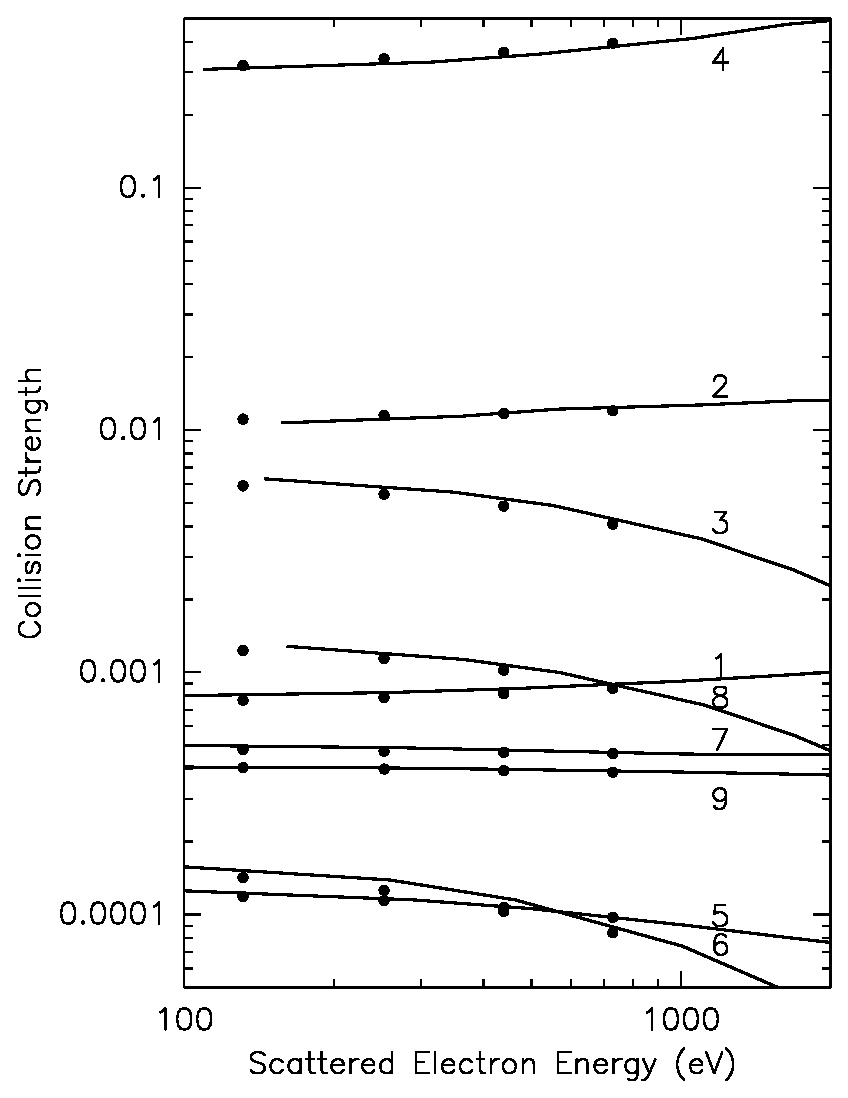
\includegraphics[width=5in]{exc.eps}
\end{figure}

\section{Conclusions}
\label{sec_conclusions}
We have presented an efficient and accurate implementation of the relativistic
DW approximation for the calculation of EIE cross sections. Special care has
been taken to account for the oscillatory behavior of the continuum
wavefunctions at large radial distances and to ensure the convergence of
partial wave summation. Sample calculations for the
$2\to 3$ transitions of Ne-like iron show good agreement with previous works.

\begin{acknowledgments}
The author would like to thank Masao Sako for his continuous test of the code
, Ehud Behar and Peter Beiersdorfer for their helpful suggestions. This work
is supported by NASA through Chandra Postdoctoral Fellowship Award Number
PF01-10014 issued by 
the Chandra X-ray Observatory Center, which is operated by Smithsonian
Astrophysical Observatory for and on behalf of NASA under contract NAS8-39073.
\end{acknowledgments}

\bibliographystyle{apsrev}
\bibliography{facref}

\end{document}
